\documentclass[11pt]{article}
\usepackage[margin=1in]{geometry}
\usepackage{amsmath,amssymb,graphicx,microtype,booktabs}
\usepackage[font=small,skip=3pt]{caption}
\usepackage[hidelinks]{hyperref}
\usepackage{enumitem}
\setlist{nosep,leftmargin=1.2em}
\setlength{\parindent}{0pt}
\setlength{\parskip}{2.5pt plus 1pt minus 1pt}
\setlength{\textfloatsep}{5pt plus 2pt minus 2pt}
\setlength{\intextsep}{7pt plus 2pt minus 2pt}
\title{\vspace{-1.6em}\textbf{What Statements Know, What Proofs Do}\vspace{-0.5em}}
\author{J. R. Landers\\[-1pt]\small Semantic views of LeanDojo Benchmark 4}
\date{\vspace{-1.2em}}

\begin{document}
\maketitle
\vspace{-1.6em}

A formal theorem has two pieces of mathematical language: its statement says what is true, and
its proof records one way to make that truth explicit.  Correctness links them, but their empirical
geometries may differ.  Similar statements may invite different arguments, while one proof idiom
can cross algebra, topology, and combinatorics.

Feature models encode that distinction deliberately: tactic names measure procedure, and cited
premises measure subject.  General-purpose embeddings offer a less supervised test, mapping raw
Lean declarations and tactic scripts into a common numerical language.  If learned semantics
erased the distinction, statement and proof clusters would agree; if it preserved their different
vocabularies, each view would recover different structure.

Three embedding experiments on the same 10,000 human-written Lean 4 proofs support the second
picture, with a warning: the geometry is meaningful but not strongly discrete.  Statement vectors
recover mathematical neighborhoods, proof vectors recover procedural modes, and their cluster
labels have adjusted mutual information only $0.080$.

\paragraph{Three semantic views.}
From 52,187 theorem records with nonempty tactic traces in the benchmark's random split, a seed-0
uniform sample selects $n=10{,}000$ records, indexed by $i\in\{1,\ldots,n\}$.  Let $s_i$ be
the complete Lean declaration without proof, $p_i$ the newline-joined traced tactic script, and
$q_i=s_i\mathbin\Vert p_i$ their labeled concatenation.  Fixed prefixes identify the fields as
``Lean 4 theorem statement'' and ``Lean 4 tactic proof.''  If $\Sigma^*$ is the set of finite
strings over the model's token alphabet, a single learned embedding map is
\[
 f:\Sigma^*\longrightarrow\mathbb{R}^{1024},\qquad
 x_i^{(v)}=\frac{f(t_i^{(v)})}{\lVert f(t_i^{(v)})\rVert_2},
 \quad v\in\{S,P,J\},
\]
Here $f$ is the encoder, $\mathbb{R}^{1024}$ is the space of 1,024-component real vectors, and
$\lVert u\rVert_2=(\sum_{j=1}^{1024}u_j^2)^{1/2}$ is the Euclidean norm.  The view labels $S,P,J$
mean statement, proof, and joint, so $t_i^{(S)}=s_i$, $t_i^{(P)}=p_i$, $t_i^{(J)}=q_i$, and
$x_i^{(v)}$ is the resulting unit vector.  Cohere Embed v4's clustering mode produces
three $10{,}000\times1{,}024$ matrices; their inputs, vectors, sampling indices, and hashes are archived.

For candidate cluster count $K\in\{4,6,8,10,12,14,16\}$ and view $v$, let
$z_i\in\{1,\ldots,K\}$ assign record $i$ and let $\mu_k^{(v)}\in\mathbb{R}^{1024}$ be cluster $k$'s
centroid in that view.  Each view minimizes the Euclidean centroid objective
\[
 \min_{z_1,\ldots,z_n,\,\mu_1,\ldots,\mu_K}
 \sum_{i=1}^n\bigl\lVert x_i^{(v)}-\mu_{z_i}^{(v)}\bigr\rVert_2^2.
\]
If $\theta$ is the angle between two unit vectors, their squared distance is
$2(1-\cos\theta)$; proximity is therefore angular as well as Euclidean, but remains empirical
rather than logical.  Definitionally equal Lean terms need not receive equal vectors.

Cluster selection is fixed before cross-view comparison.  Adjusted mutual information (AMI) is
label-permutation-invariant agreement corrected for chance: for fixed cluster sizes its random
expectation is zero, while identical partitions score one.  Let $z^{(v,K)}$ be full-data labels,
$z_r^{(v,K)}$ labels fitted on 80\% subset $I_r$, and $z|_{I_r}$ the restriction to it.  Stability
over four independent subsamples is
\[
 A_K^{(v)}=\frac14\sum_{r=1}^4
 \operatorname{AMI}\!\left(z^{(v,K)}|_{I_r},z_r^{(v,K)}\right).
\]
Cosine silhouette is the $[-1,1]$ contrast between mean within-cluster cosine distance and the
nearest other-cluster mean, averaged over a fixed 2,000 records.  The rule selects the largest
silhouette among candidates with $A_K^{(v)}\geq0.8$, or maximum stability if none qualify.  No view
qualifies; the fallbacks are $K_S=16$, $K_P=4$, and $K_J=16$ (stabilities $0.416$, $0.622$, $0.477$;
silhouettes $0.031$, $0.076$, $0.031$).  These are comparison resolutions, not true category counts.

\begin{figure}[t]
  \centering
  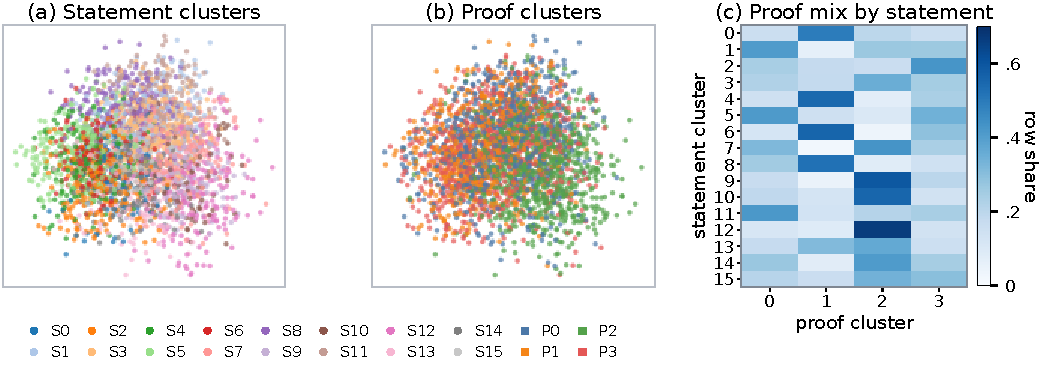
\includegraphics[width=\textwidth]{semantic_comparison.pdf}
  \caption{A fixed 3,000-record sample in the statement-embedding principal-component analysis
  (PCA) plane, colored by statement cluster (a) and proof cluster (b), with the full row-normalized
  statement--proof table (c).  PCA is illustrative: all fits and statistics use all 1,024 coordinates
  and 10,000 records.  Statement clusters organize their plane; proof modes cut across it.}
  \label{fig:semantic}
\end{figure}

\paragraph{Comparing learned partitions.}
For labelings $A$ and $B$ with cluster indices $a$ and $b$, let
$N_{ab}=|\{i:A_i=a,B_i=b\}|$, $p_{ab}=N_{ab}/n$, $p_{a+}=\sum_b p_{ab}$, and
$p_{+b}=\sum_a p_{ab}$.  Write $H(A)=-\sum_a p_{a+}\log p_{a+}$ for Shannon entropy and analogously
for $H(B)$, using natural logarithms.  Mutual information (MI) and its normalized form (NMI) are
\[
 I(A;B)=\sum_{a,b:p_{ab}>0}p_{ab}\log\frac{p_{ab}}{p_{a+}p_{+b}},
 \qquad
 \operatorname{NMI}(A,B)=\frac{I(A;B)}{\sqrt{H(A)H(B)}}.
\]
AMI subtracts the expected mutual information under fixed cluster sizes and scales by the
corresponding entropy ceiling \cite{vinh}.  For marginal counts
$N_{a+}=\sum_bN_{ab}$ and $N_{+b}=\sum_aN_{ab}$, Cram\'er's $V$ is
\[
 V=\sqrt{\frac{\chi^2}{n\min(K_A-1,K_B-1)}},\qquad
 \chi^2=\sum_{a,b}\frac{(N_{ab}-N_{a+}N_{+b}/n)^2}{N_{a+}N_{+b}/n},
\]
where $\chi^2$ is Pearson's chi-squared statistic and $K_A,K_B$ are the numbers of clusters.
$V$ emphasizes cellwise departures rather than information shared across the full partitions;
neither measure depends on Figure~\ref{fig:semantic}'s projection.

Statement and proof clusters have AMI $0.080$, NMI $0.081$, and $V=0.337$: detectable
correspondence, but different partitions.  Statement clusters collect category theory, lists,
probability, calculus, and algebraic structure; proof clusters separate short simplification
(2,494 records, mean 1.43 tactics) and rewriting proofs (2,446, mean 1.84) from two structured
modes (means 5.71 and 7.45) rich in \texttt{have}, \texttt{apply}, \texttt{refine'}, \texttt{intro},
and \texttt{exact}.

The joint embedding favors statements: its AMI is $0.362$ with statement clusters but $0.152$ with
proof clusters.  Unlike a linear average, a transformer can weight its input fields unequally.

\paragraph{External checks.}
An earlier same-sample analysis defined style from tactic-head unigrams and bigrams, and domain
from cited premises \cite{textures}.  Its style--domain AMI was $0.015$; module AMI was $0.025$ for
style versus $0.241$ for domain.  Embeddings preserve that asymmetry:
\[
\begin{array}{lccc}
\toprule
\text{embedding view} & \text{feature style AMI} & \text{feature domain AMI} & \text{module AMI}\\
\midrule
\text{statement} & 0.032 & 0.165 & 0.187\\
\text{proof}     & 0.209 & 0.060 & 0.045\\
\text{joint}     & 0.063 & 0.209 & 0.203\\
\bottomrule
\end{array}
\]
Because embeddings never see those topic labels, this is an external check: statements prefer
domain, proofs prefer style, and joint vectors act like statements.  Content follows the source
hierarchy; procedure travels across it.

\paragraph{Reading the map.}
The larger statement--proof AMI does not reverse the feature result.  Names occur in proofs and
declarations suggest tactics, so embeddings detect local associations while global partitions
remain distinct \cite{graph2tac,leandojo}.  Near-zero silhouettes and subsample AMI below $0.8$
likewise indicate overlapping neighborhoods, not isolated species: readable clusters summarize
geometry, and nearby resolutions remain plausible.

A sharper test would compare renamings, equivalent statements, or multiple proofs.  For balance
weight $0\leq\alpha\leq1$, define the late-fusion vector
\[
 y_i(\alpha)=
 \frac{\alpha x_i^{(S)}+(1-\alpha)x_i^{(P)}}
 {\lVert\alpha x_i^{(S)}+(1-\alpha)x_i^{(P)}\rVert_2},
\]
Varying $\alpha$ traces alignment changes; neighbor tests could separate shared premises, proof
plans, and surface vocabulary.

\paragraph{Limitations and interpretation.}
This code/text encoder is not the Lean kernel, so similarity is empirical, not logical.  The sample
omits untraced declarations; short proofs and automation hide reasoning; modules are coarse.  All
30,000 vectors and hashes are retained for reproduction.

The negative result is informative: a learned map preserves the porous boundary between content
and procedure.  Statements know where mathematics lives; proofs show how arguments move through it.

\begin{thebibliography}{9}\scriptsize
\setlength{\itemsep}{0pt}
\bibitem{textures} J. R. Landers. ``Textures of Modern Formal Mathematics.'' Remarks on LeanDojo Benchmark 4, 2026.
\bibitem{leandojo} K. Yang et al. ``LeanDojo: Theorem Proving with Retrieval-Augmented Language Models.'' NeurIPS Datasets and Benchmarks, 2023.
\bibitem{graph2tac} L. Blaauwbroek et al. ``Graph2Tac: Online Representation Learning of Formal Math Concepts.'' arXiv:2401.02949, 2024.
\bibitem{vinh} N. X. Vinh, J. Epps, and J. Bailey. ``Information Theoretic Measures for Clusterings Comparison.'' JMLR 11, pp. 2837--2854, 2010.
\end{thebibliography}

\end{document}
